\section{DRTA sonda}
    \subsection{Princip fungování} \label{sec:DRTA-princip}
        Myšlenka stojící za DRTA sondou se opírá právě o měření rovnovážných teplot (viz předchozí Kapitola \ref{sec:mereni-teplot}). Budeme-li uvažovat teplotní čidlo s restitučním faktorem $f_A$, pak bude měřená teplota $T_{rA}$ dána následovně:
        \begin{equation} \label{eq:trA}
            T_{rA} = T + f_A \frac{u^2}{2 c_p}
        \end{equation}
        \noindent Jednoduchou úpravou lze odvodit vztah pro určení rychlosti proudění:
        \begin{equation} \label{eq:rychlost-jenom-A}
            u = \sqrt{2 c_p \frac{T_{rA} - T}{f_A}}
        \end{equation}
        Takový postup by však vyžadoval znalost statické teploty nabíhajícího proudu $T$, nebo potažmo teploty klidové $T_0$ – tuto metodiku lze najít v řadě aplikací (viz metoda RTA – \textit{Recovery Temperature Anemometry} \cite{Ishibashi2004, Ishibashi2012}). Zde byl k měření použit termočlánek s restitučním faktorem uvažovaným jako $\sqrt{Pr}$ a výsledná rychlost proudění byla stanovena ze vztahu:
        \begin{equation}
            u = \sqrt{\frac{2 \kappa r}{\kappa - 1} \frac{T_0 - T_{rA}}{f_A}}
        \end{equation}
        
        Nevýhodou výše uvedené RTA metody je právě nutnost měření dalších parametrů proudění ($T$, $T_0$), což značně omezuje možnosti jejího využití. Klíčovým krokem v návrhu DRTA sondy je proto eliminace statické teploty ze Vztahu \ref{eq:rychlost-jenom-A}. Toho lze docílit použitím odlišného teplotního čidla – odlišnost je zde reprezentovaná rozdílným restitučním faktorem, který označme $f_B$. Toto čidlo bude tedy indikovat teplotu $T_{rB}$:
        \begin{equation} \label{eq:trB}
            T_{rB} = T + f_B \frac{u^2}{2 c_p}
        \end{equation}
        \noindent Rychlost proudění lze následně určit z rozdílu Vztahů \ref{eq:trA} a \ref{eq:trB}:
        \begin{align} \label{eq:mereni-rychlosti}
                T_{rA} - T_{rB} &= \brac{f_A - f_b} \frac{u^2}{2 c_p} \\
                u &= \sqrt{\frac{2 c_p \brac{T_{rA} - T_{rB}}}{\brac{f_A - f_B}}}
        \end{align}

        Výhoda použití dvou teplotních snímačů s rozdílnými restitučními faktory spočívá navíc v tom, že lze obdobně odvodit i vztahy pro určení Machova čísla a statické teploty nabíhajícího proudu. Pro určení $\Ma$ je třeba nejprve upravit Vztahy \ref{eq:trA} a \ref{eq:trB}:
        \begin{align}
            \begin{split}
                T_{rA} &= T + f_A \frac{u^2}{2 c_p} \frac{a^2}{a^2} = T \brac{1 + f_A \frac{\kappa - 1}{2} \Ma ^2} \\
                T_{rB} &=  T \brac{1 + f_B \frac{\kappa - 1}{2} \Ma ^2}
            \end{split}
        \end{align}
        \noindent Výsledný vztah pro $\Ma$ vznikne z podílu měřených teplot:
        \begin{align}
            \begin{split}
                \frac{T_{rA}}{T_{rB}} &= \frac{1 + f_A \frac{\kappa - 1}{2} \Ma ^2}{1 + f_B \frac{\kappa - 1}{2} \Ma ^2} \\
                \Ma &= \sqrt{\frac{2}{\kappa - 1} \frac{T_{rA}-T_{rB}}{T_{rB} f_A - T_{rA} f_B}}
            \end{split}
        \end{align}
        \noindent Určení statické teploty lze odvodit pomocí eliminace rychosti proudění ze Vztahů \ref{eq:trA} a \ref{eq:trB}:
        \begin{align}
            \begin{split}
                \frac{u^2}{2 c_p} &= \frac{T_{rA} - T}{f_A} = \frac{T_{rB} - T}{f_B} \\
                T &= \frac{T_{rB} f_A - T_{rA} f_B}{f_A - f_B}
            \end{split}
        \end{align}

    \subsection{Výchozí geometrie}
        Jak již vyplývá z principu fungování DRTA sondy, klíčovými prvky konstrukce jsou dvě teplotní čidla. V tomto případě byly zvoleny odporové teplotní snímače Pt100 (model \textit{1PT100K2515} značky Omega Engineering) o průměru $1.5 \Unit{mm}$ a délce $25 \Unit{mm}$. Ty jsou uchyceny pomocí těsnění v mosazné trubici o vnějším průměru $4 \Unit{mm}$ a tloušťce stěny $0.4 \Unit{mm}$. Výchozí geometrie sondy je patrná z Obrázku \ref{fig:vychozi-DRTA}, detailní rozměry jsou poté uvedeny v Příloze \ref{fig:sonda-bez-stineni-B-vykres}.

        \begin{figure}[ht!]
            \centering
            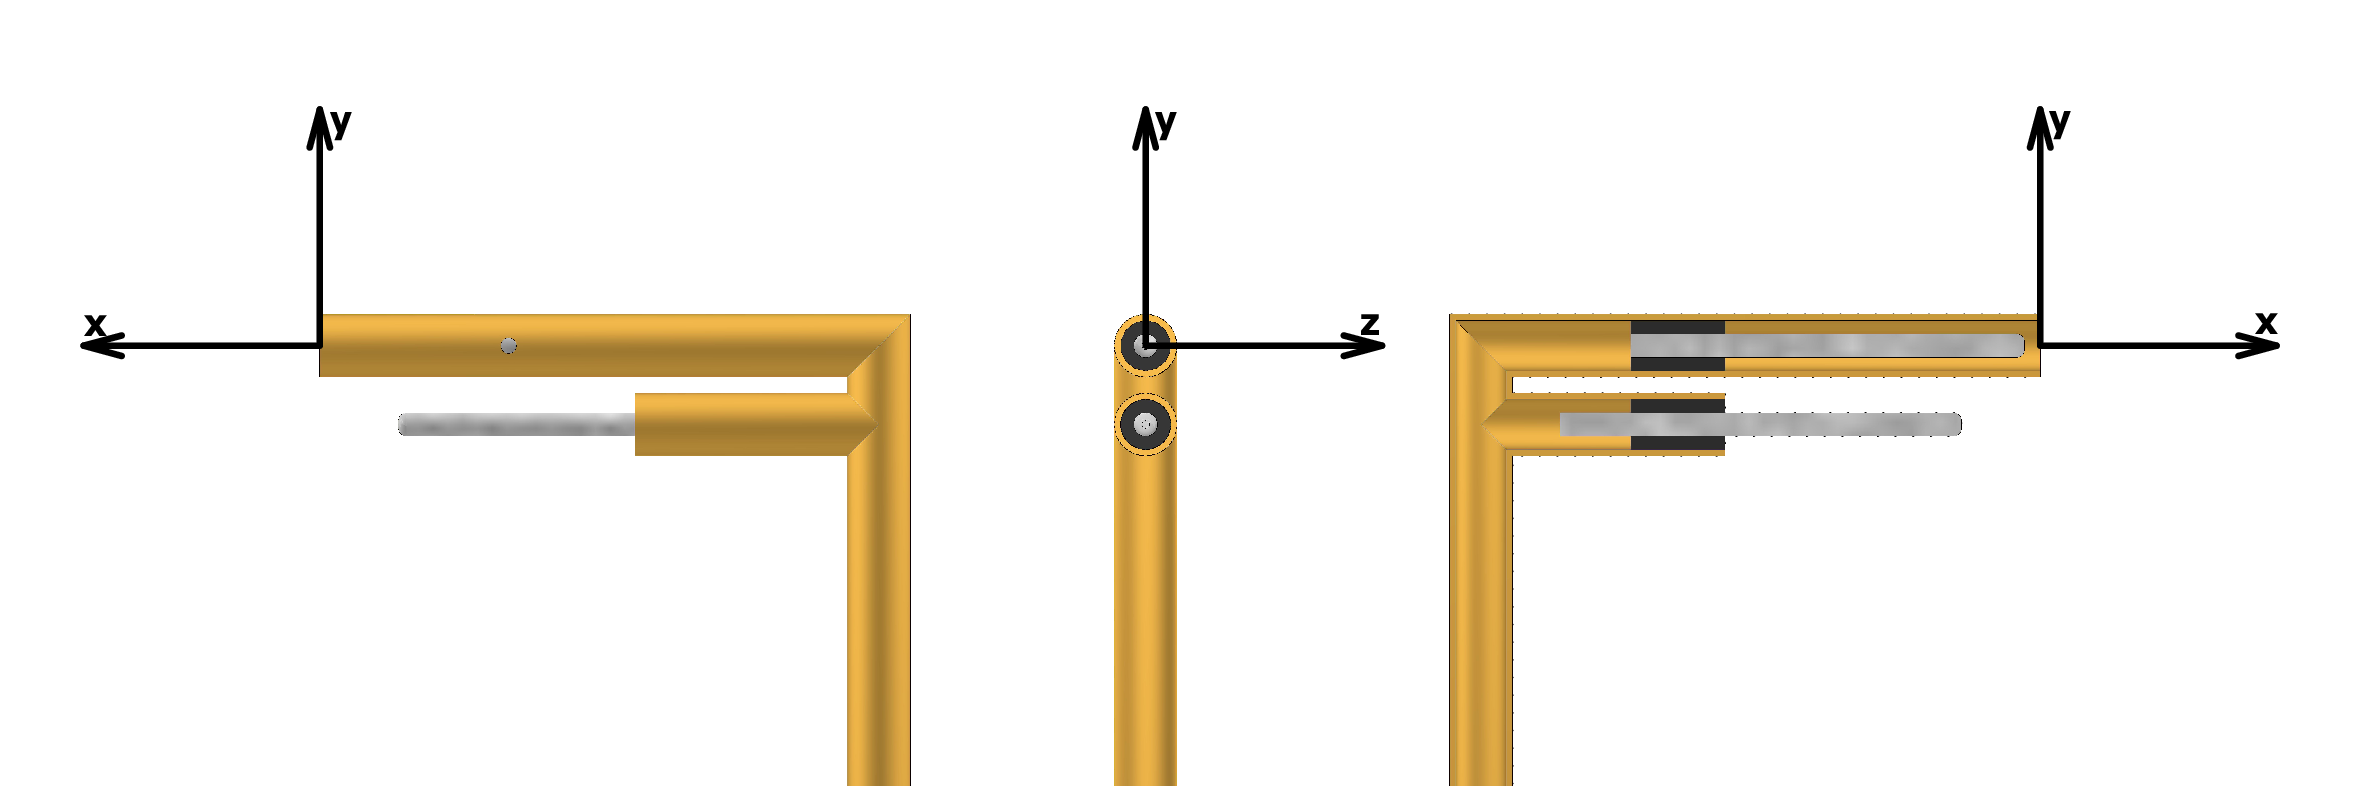
\includegraphics[width=\textwidth]{200_DRTA_SONDA/Vychozi_DRTA.png}
            \caption{Výchozí geometrie DRTA sondy.}
            \label{fig:vychozi-DRTA}
        \end{figure}

        Klíčový je zde rozdíl restitučních faktorů teplotních čidel. To je zajištěno opláštěním jednoho z nich – bude značeno jako čidlo A. Při proudění plynu stínicí trubicí dochází k jeho výraznému zpomalení, což vede k nárůstu statické teploty a čidlo se tak zahřívá více, než kdyby bylo umístěné volně v proudu. Stínění je opatřeno dvěma ventilačními otvory o průměru $1 \Unit{mm}$, které zajišťují proudění vzduchu trubicí. Konstrukce čidla A se tak podobá měření stagnační teploty (viz Kapitola \ref{sec:mereni-teplot}), kdy je cílem se co nejvíce přiblížit stavu $f_A \rightarrow 1$.
        \clearpage
        
    \subsection{Cíle numerických simulací}
        Hlavním cílem CFD simulací byla úprava geometrie sondy tak, aby byla zajištěna její co největší směrová necitlivost a zároveň použitelnost nezávisle na rychlosti proudění. Návrhy byly prováděny pro vysoké podzvukové rychlosti. Dalším cílem bylo dále dosažení co nejvyššího rozdílu restitučních faktorů s ohledem na další zvolené úpravy geometrie.

        Charakter konstrukčních úprav se odvíjel také od snahy zachovat původní koncept sondy a měl umožnit pozdější snadnou konstrukci nového modelu pro experimentální testování.